\documentclass[tikz,border=4pt]{standalone}
\usepackage{mathptmx}          % Times for text and math
\usepackage[T1]{fontenc}
\usepackage{amsmath}
\usetikzlibrary{arrows.meta,calc}

\definecolor{inp}{HTML}{EAF0F8}
\definecolor{grf}{HTML}{E9F4EC}
\definecolor{adp}{HTML}{FFF3E0}
\definecolor{mdl}{HTML}{F1EBF7}
\definecolor{obj}{HTML}{FBECEC}
\definecolor{dia}{HTML}{F3F3F3}
\definecolor{edgeR}{HTML}{2F6DB5}
\definecolor{edgeT}{HTML}{C0392B}

\tikzset{
  font=\small,
  panel/.style={draw=black!55, rounded corners=3pt, line width=0.6pt},
  ptitle/.style={font=\small\bfseries, anchor=north west, inner sep=0pt},
  box/.style={draw=black!55, rounded corners=2pt, fill=white, align=center, inner sep=3pt, font=\footnotesize},
  flow/.style={-{Latex[length=2.6mm]}, line width=0.9pt, black!75},
  thin/.style={-{Latex[length=1.8mm]}, line width=0.5pt, black!60},
  evals/.style={-{Latex[length=1.8mm]}, line width=0.6pt, dashed, black!55},
  fnode/.style={circle, draw=black!70, fill=white, minimum size=4.4mm, inner sep=0pt, font=\scriptsize},
  anode/.style={fnode, fill=edgeT!20, draw=edgeT},
}

\begin{document}
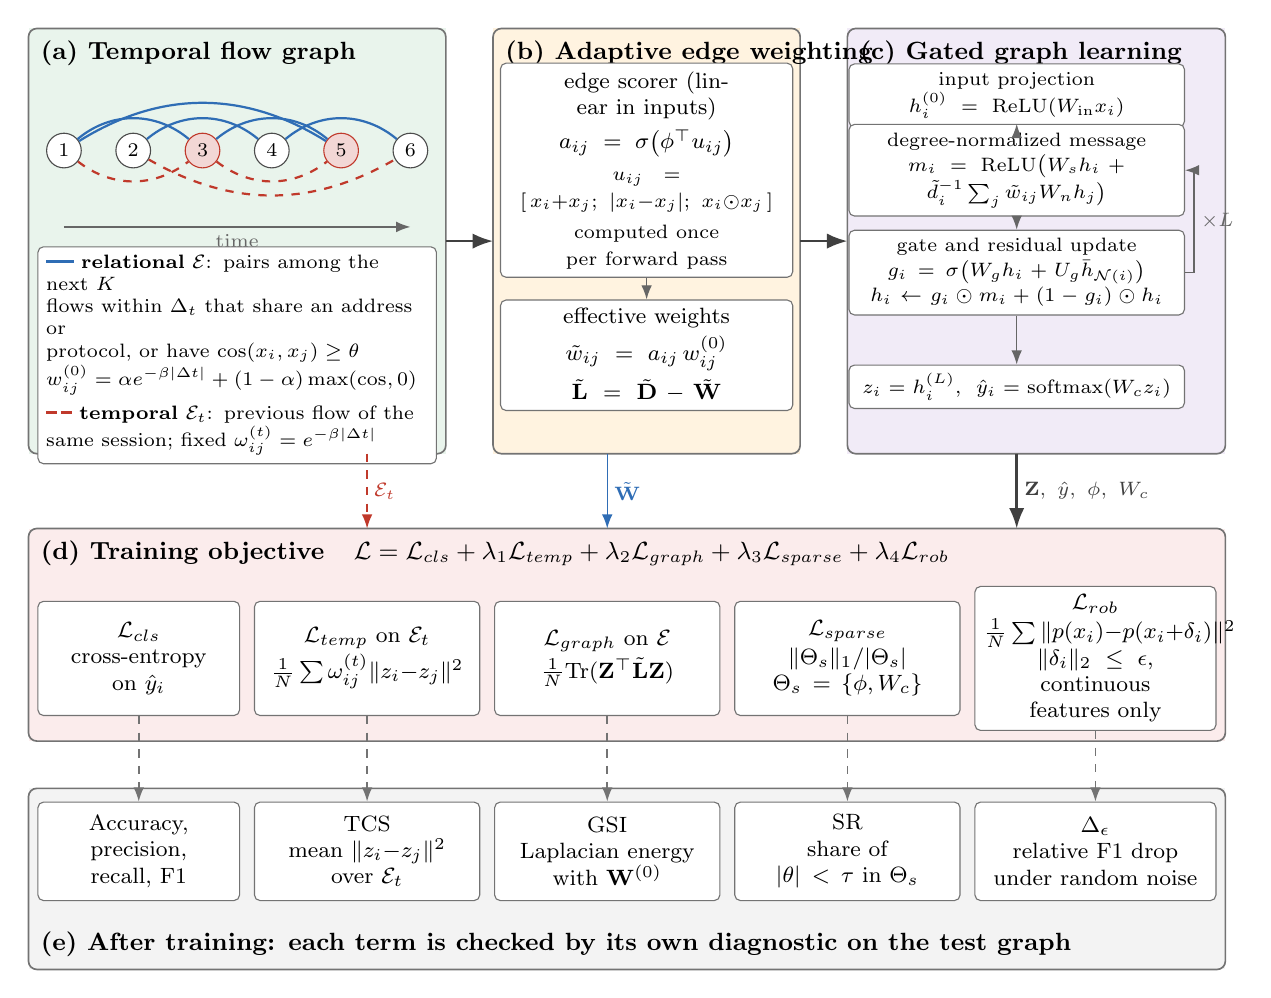
\begin{tikzpicture}

% ============================================================ row 1: panels
\begin{scope}[xshift=-4.5cm]
\fill[grf] (4.5,0) rectangle (9.8,5.4); \draw[panel] (4.5,0) rectangle (9.8,5.4);
\fill[adp] (10.4,0) rectangle (14.3,5.4); \draw[panel] (10.4,0) rectangle (14.3,5.4);
\fill[mdl] (14.9,0) rectangle (19.7,5.4); \draw[panel] (14.9,0) rectangle (19.7,5.4);
\node[ptitle] at (4.65,5.25) {(a) Temporal flow graph};
\node[ptitle] at (10.55,5.25) {(b) Adaptive edge weighting};
\node[ptitle] at (15.05,5.25) {(c) Gated graph learning};

% ---------------- (a) graph: flows in time order; shaded = attack
\foreach \i/\k in {1/0,2/0,3/1,4/0,5/1,6/0}{
  \pgfmathsetmacro{\xx}{4.95+(\i-1)*0.88}
  \ifnum\k=1 \node[anode] (n\i) at (\xx,3.85) {\i}; \else \node[fnode] (n\i) at (\xx,3.85) {\i}; \fi}
\draw[edgeR, line width=0.8pt] (n1) to[bend left=40] (n3);
\draw[edgeR, line width=0.8pt] (n2) to[bend left=40] (n4);
\draw[edgeR, line width=0.8pt] (n4) to[bend left=40] (n6);
\draw[edgeR, line width=0.8pt] (n3) to[bend left=40] (n5);
\draw[edgeR, line width=0.8pt] (n1) to[bend left=32] (n5);
\draw[edgeT, line width=0.8pt, dashed] (n1) to[bend right=38] (n3);
\draw[edgeT, line width=0.8pt, dashed] (n3) to[bend right=38] (n5);
\draw[edgeT, line width=0.8pt, dashed] (n2) to[bend right=30] (n6);
\draw[thin] (4.95,2.88) -- node[below=-1pt, font=\scriptsize]{time} (9.35,2.88);
\node[box, text width=4.85cm, align=left, font=\scriptsize] at (7.15,1.25) {%
  \textcolor{edgeR}{\rule[2pt]{10pt}{1pt}}\ \textbf{relational} $\mathcal{E}$: pairs among the next $K$\\
  flows within $\Delta_t$ that share an address or\\
  protocol, or have $\cos(x_i,x_j)\ge\theta$\\
  $w^{(0)}_{ij}=\alpha e^{-\beta|\Delta t|}+(1-\alpha)\max(\cos,0)$\\[3pt]
  \textcolor{edgeT}{\rule[2pt]{4pt}{1pt}\,\rule[2pt]{4pt}{1pt}}\ \textbf{temporal} $\mathcal{E}_t$: previous flow of the\\
  same session; fixed $\omega^{(t)}_{ij}=e^{-\beta|\Delta t|}$};

% ---------------- (b)
\node[box, text width=3.5cm] (sc) at (12.35,3.6) {%
  edge scorer (linear in inputs)\\[3pt]
  $a_{ij}=\sigma\big(\phi^{\top}u_{ij}\big)$\\[2pt]
  {\scriptsize $u_{ij}=[\,x_i{+}x_j;\ |x_i{-}x_j|;\ x_i{\odot}x_j\,]$}\\[2pt]
  {\scriptsize computed once per forward pass}};
\node[box, text width=3.5cm] (we) at (12.35,1.25) {%
  effective weights\\[2pt]
  $\tilde w_{ij}=a_{ij}\,w^{(0)}_{ij}$\\[2pt]
  $\tilde{\mathbf L}=\tilde{\mathbf D}-\tilde{\mathbf W}$};
\draw[thin] (sc) -- (we);

% ---------------- (c)
\begin{scope}[box/.append style={font=\scriptsize, text width=4.05cm}]
\node[box] (h0) at (17.05,4.55) {input projection\ \ $h^{(0)}_i=\mathrm{ReLU}(W_{\mathrm{in}}x_i)$};
\node[box] (msg) at (17.05,3.6) {degree-normalized message\\[1pt] $m_i=\mathrm{ReLU}\big(W_s h_i+\tilde d_i^{-1}\sum_j \tilde w_{ij}W_n h_j\big)$};
\node[box] (gate) at (17.05,2.3) {gate and residual update\\[1pt] $g_i=\sigma\big(W_g h_i+U_g\bar h_{\mathcal N(i)}\big)$\\[1pt] $h_i\leftarrow g_i\odot m_i+(1-g_i)\odot h_i$};
\node[box] (cls) at (17.05,0.85) {$z_i=h^{(L)}_i$,\ \ $\hat y_i=\mathrm{softmax}(W_c z_i)$};
\end{scope}
\draw[thin] (h0) -- (msg); \draw[thin] (msg) -- (gate); \draw[thin] (gate) -- (cls);
\draw[thin] (gate.east) -- (19.3,2.3) -- node[right=-1pt, font=\scriptsize, pos=0.5]{$\times L$} (19.3,3.6) -- (msg.east);

% ---------------- arrows between panels
\draw[flow] (9.8,2.7) -- (10.4,2.7);
\draw[flow] (14.3,2.7) -- (14.9,2.7);

\end{scope}

% ============================================================ row 2: objective
\fill[obj] (0,-3.65) rectangle (15.2,-0.95); \draw[panel] (0,-3.65) rectangle (15.2,-0.95);
\node[ptitle] at (0.15,-1.1) {(d) Training objective\quad
  $\mathcal L=\mathcal L_{cls}+\lambda_1\mathcal L_{temp}+\lambda_2\mathcal L_{graph}+\lambda_3\mathcal L_{sparse}+\lambda_4\mathcal L_{rob}$};
\def\yo{-2.6}
\begin{scope}[box/.append style={minimum height=1.45cm}]
\node[box, text width=2.35cm] (Lc) at (1.40,\yo) {$\mathcal L_{cls}$\\ cross-entropy\\ on $\hat y_i$};
\node[box, text width=2.65cm] (Lt) at (4.30,\yo) {$\mathcal L_{temp}$ on $\mathcal E_t$\\[1pt] $\frac1N\sum\omega^{(t)}_{ij}\|z_i{-}z_j\|^2$};
\node[box, text width=2.65cm] (Lg) at (7.35,\yo) {$\mathcal L_{graph}$ on $\mathcal E$\\[1pt] $\frac1N\mathrm{Tr}(\mathbf Z^{\top}\tilde{\mathbf L}\mathbf Z)$};
\node[box, text width=2.65cm] (Ls) at (10.40,\yo) {$\mathcal L_{sparse}$\\[1pt] $\|\Theta_s\|_1/|\Theta_s|$\\ $\Theta_s=\{\phi,W_c\}$};
\node[box, text width=2.85cm] (Lr) at (13.55,\yo) {$\mathcal L_{rob}$\\[1pt] $\frac1N\sum\|p(x_i){-}p(x_i{+}\delta_i)\|^2$\\ $\|\delta_i\|_2\le\epsilon$,\\ continuous features only};
\end{scope}

% what each term reads from the model (arrows across the gap only)
\draw[thin, edgeT, dashed] (4.30,0) -- node[right=-1pt, font=\scriptsize]{$\mathcal E_t$} (4.30,-0.95);
\draw[thin, edgeR] (7.35,0) -- node[right=-1pt, font=\scriptsize]{$\tilde{\mathbf W}$} (7.35,-0.95);
\draw[flow] (12.55,0) -- node[right=-1pt, font=\scriptsize]{$\mathbf Z,\ \hat y,\ \phi,\ W_c$} (12.55,-0.95);

% ============================================================ row 3: diagnostics
\fill[dia] (0,-6.55) rectangle (15.2,-4.25); \draw[panel] (0,-6.55) rectangle (15.2,-4.25);
\def\yd{-5.05}
\begin{scope}[box/.append style={minimum height=1.25cm}]
\node[box, text width=2.35cm] (Dc) at (1.40,\yd) {Accuracy, precision,\\ recall, F1};
\node[box, text width=2.65cm] (Dt) at (4.30,\yd) {TCS\\ mean $\|z_i{-}z_j\|^2$\\ over $\mathcal E_t$};
\node[box, text width=2.65cm] (Dg) at (7.35,\yd) {GSI\\ Laplacian energy\\ with $\mathbf W^{(0)}$};
\node[box, text width=2.65cm] (Ds) at (10.40,\yd) {SR\\ share of $|\theta|<\tau$ in $\Theta_s$};
\node[box, text width=2.85cm] (Dr) at (13.55,\yd) {$\Delta_\epsilon$\\ relative F1 drop\\ under random noise};
\end{scope}
\foreach \a/\b in {Lc/Dc, Lt/Dt, Lg/Dg, Ls/Ds, Lr/Dr} \draw[evals] (\a.south) -- (\b.north);
\node[ptitle, anchor=south west] at (0.15,-6.4) {(e) After training: each term is checked by its own diagnostic on the test graph};

\end{tikzpicture}
\end{document}
